%%% Local Variables: ***

\subsection{Results}

\subsubsection{Post Test Check}

For each stimulus set used in the experiment,
participants correctly said that the base species
and the correct response species 
belonged to the same taxonomic group (accuracy > 70.5\%, p's < .01),
and that the moderate and strong foils
had the appropriate relationship (food chain or shared habitat)
with their base species (accuracy > 75\%, p's < .001).
Therefore, no data were excluded from the analyses on these criteria.
Full post-test results can be found in Appendix~\ref{appendix:exp4_posttest}.

\subsubsection{Reasoning Accuracy}

In order to analyse data from the reasoning trials,
for each trial I divided that participants' rating of
the association between the base and the correct species
by their rating of the association between the base and the foil.
This produced a ratio reflecting the extent to which
that participants' associative knowledge
favoured one or other response option.
Values of this ratio ranged from $\frac{1}{9}$
($.111$; association of 1 for the correct species, and 9 for the foil),
to $\frac{1}{1}$ (equal association for both species),
to $\frac{9}{1}$
(association of 9 for the correct species, and 1 for the foil).

For each analysis, I log-transformed this ratio
to create a normally-distributed linear predictor,
as is standard practice when using ratios as regression predictors \citep{Gelman2007}.
Note that $log(\frac{1}{1}) = 0$,
and correspondingly $log(\frac{>1}{1}) > 0$ and $log(\frac{1}{>1}) < 0$
(see Figure~\ref{fig:exp4_log_transform}).
Therefore, when using the log-transformed ratio as a predictor,
a positive regression weight means that
the dependent variable is greater/more likely when the ratio is greater than $\frac{1}{1}$,
or in other words, when the association rating favours the correct response.

\begin{figure}[h]
  \centering
  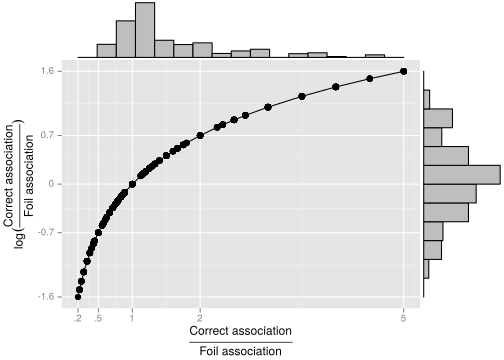
\includegraphics[width=.7\textwidth]{imgs/exp4_log_transform.pdf}
  \caption[The log-transformed association ratio, used as a predictor in Experiment 4.]{
    To analyse data from Experiment 4,
    each participants' rating for the association between
    the base species and the correct response species
    was divided by their rating for
    the base and the foil species, to form an association ratio.
    These ratios were log-transformed to use as predictors in regression analyses:
    after log-transformation, the difference between 1 and 0.2 (dividing by five)
    is the same as the difference between 1 and 5 (multiplying by five).
    \label{fig:exp4_log_transform}
  }
\end{figure}

Some aspects of the analyses based on this ratio are slightly unusual,
and so I will go through my first analysis,
predicting participants' responses,
in detail to familiarise readers with the method.
Figure~\ref{fig:exp4_ratio_accuracy} plots the proportion of correct responses 
(choosing the species belonging to the same taxonomic group as the base) given, on the y axis,
as a function of the association ratio, on the x axis.
Note that the x axis is log-scaled.
For plotting, I have divided the log-transformed ratio into 13 equal bins,
and plotted the mean and standard error of the dependent variable within each bin.
For the analyses, I fit log-linear, or logistic mixed models,
with random intercepts for each participant, and for each stimulus set.
The log-transformed association ratio from each trial was used as the predictor in the models.

\begin{figure}[h]
  \centering
  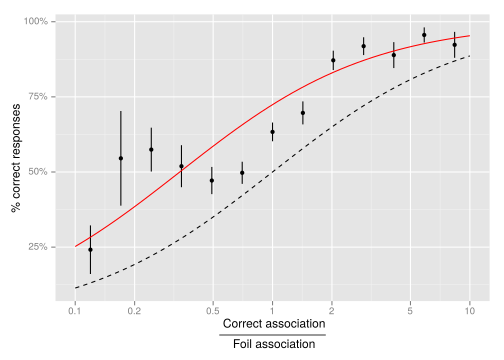
\includegraphics[width=.6\textwidth]{imgs/exp4_ratio_accuracy.pdf}
  \caption[Effect of the association ratio of participants' accuracy, Experiment 4.]{
    Correct responses on Experiment 4, as a function of
    the association ratio in favour of the correct species.
    As the ratio increased in favour of the correct species,
    participants became more likely to select that species.
    The fitted model (red line) included a significant positive intercept term,
    meaning that participants were more likely to select the correct species
    than would be predicted based on the association ratio alone (dashed black line).
    \label{fig:exp4_ratio_accuracy}
  }
\end{figure}

The association ratio was a significant predictor of the odds of a correct response
($\beta$ = 0.89, CI = [0.68, 1.1], z = 8.604, p < .0001).
Interpretation of the regression $\beta$ here is not straightforward,
but positive $\beta$s indicate that the dependent variable
(odds of a correct response) was positively related to
the size of the association ratio in favour of the correct response.
Fortunately, we can simply look to the predicted values from this model
(solid red line in Figure~\ref{fig:exp4_ratio_accuracy})
to see the magnitude of this effect.

An unusual property of these models is that
the intercept parameter is also meaningful.
As the log-transformed association ratio is the only predictor in the model,
the intercept reflects the expected value
when this predictor is at 0, or in other words, for a ratio of $\frac{1}{1}$.
If participants do not make use of structured knowledge,
we would expect participants to select the correct species
50\% of the time for such trials, something that would correspond to an intercept of 0.
The dashed black line in Figure~\ref{fig:exp4_ratio_accuracy}
shows the predicted values for such a model, with intercept 0.
A significant positive intercept means that
participants were more likely to select the correct species
than would be expected from the association ratio alone,
while a negative intercept means they were less likely.
There was a significant positive intercept term in this model
($logit(\beta)$ = 72\%, CI = [56\%, 85\%], z = 2.585, p = .0010).
I report the $logit$ of the regression $\beta$ weights here
as an easily interpretable measure of how much participants
were biased towards the correct species.
In this case, $logit(\beta)$ reflects how often
participants would be expected to select the correct species
on trials where the association ratio = $\frac{1}{1}$,
according to the fitted model
(i.e. where the red line on Figure~\ref{fig:exp4_ratio_accuracy}
crosses $1$ on the x axis).
Together, these results mean that participants were
a) more likely to select the correct species when
they rated it as being more strongly associated with the base
than the foil was, and
b) biased towards the correct option rather than the foil
beyond the effect of the association ratio.

\begin{figure}[h]
  \centering
  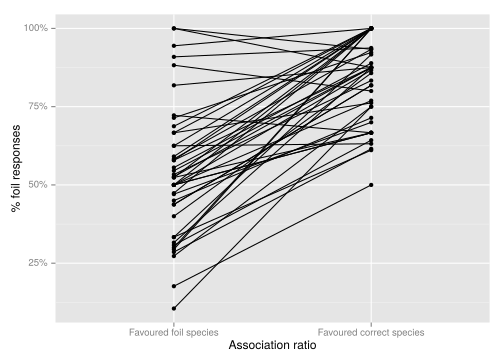
\includegraphics[width=.7\textwidth]{imgs/exp4_acc_ids.pdf}
  \caption[Proportion of correct responses
    given by each participant, by association ratio,
    in Experiment 4]{
    Participants' number of correct responses
    on trials where the association ratio favoured either
    the correct species or the foil species.
    40 of 44 participants were more likely to select the correct species
    when the association ratio favoured it
    than when the ratio favoured the foil.
    \label{fig:exp4_acc_ids} }
\end{figure}

To analyse individual differences in the number of correct responses
(Figure~\ref{fig:exp4_acc_ids}),
I calculated the number of correct responses given by each participant
both when the association ratio favoured the foil species,
and when it favoured the correct species,
excluding trials where species were rated as equally associated.
Of the 44 participants, 40 were more likely to select the correct species
when the association ratio favoured it,
and 4 were less likely to do so.
Therefore, it appears that almost all of my participants
were influenced by the association between species.

\FloatBarrier
\subsubsection{Correct Responses}

Analysing trials where the correct species was selected,
the association ratio had no effect on participants' movement initiation times
(mean = 574 msec, SD = 285; t(529.6) = 0.387, p > .6).
There was a marginally significant effect of the association ratio
on participants' response latencies
(mean RT = 1509, SD = 567;
$e^{\beta}$ = 98\%, CI = [96\%, 100.4\%], t(787.1) = 1.647, p =.100),
meaning that participants were marginally faster to respond correctly
as the association ratio in favour of the correct species increased.

Maximum deviation was once again bimodally distributed
(Bimodality Coefficient = .635; Hartigan's D = .025, N = 1188, p < .0001),
and reversal trajectories were classified
as described in Chapter 2 (MD cut-off = 0.923, see Appendix~\ref{appendix:reversals}).
Figure~\ref{fig:exp4_reversals} shows the proportion of correct responses
that were categorised as reversals ---
that is, where participants moved initially towards the foil
before selecting the correct species ---
as a function of the association ratio.
A logistic mixed model (dashed red line) showed that
participants were less likely to follow such a reversal trajectory
as the association ratio increased in favour of the correct species
($e^{\beta}$ = .8, CI = [.6, .97], z = 2.152, p = .0314).
However, the data were fit slightly better%
\footnote{
  As these two models were not nested,
  and contained the same number of parameters,
  we can identify which model best fits the data
  by comparing the deviance of each,
  but we cannot calculate p values for
  the difference between the models.
}
($\Delta$deviance = $0.715$)
by an alternative model (solid red line),
where the odds of a trajectory being classed as a reversal
when selecting the correct species
were predicted by the \emph{absolute magnitude} of the log-transformed association ratios
($e^{\beta}$ = .7, CI = [.5, .9], z = 2.289, p = .0221).
In other words, when selecting the correct species,
participants were most likely to trace a reversal trajectory
when the species were equally associated,
and less likely to do so as the ratio changed in favour of either species.
This trend may appear counter-intuitive,
but may make sense when one considers that
this analysis does not include trials where the foil species was selected.
An explanation for the trend is offered in the discussion, below.


\subsubsection{Cursor Trajectories}


As before, mouse trajectories in this experiment
can be described in terms of whether or not
they initially moved towards the correct species ($\alpha$),
whether they selected the correct species
after initially moving towards it ($\beta$),
and whether they changed direction to select the correct species
after initially moving towards the foil ($\gamma$;
see Figure~\ref{fig:exp3_transitions}).
I modelled these three parameters
using multilevel logistic regression models,
with the log-transformed association ratio
and an intercept term as predictors,
and random intercepts for each participant and stimulus set.

\begin{figure}[tp]
  \centering
  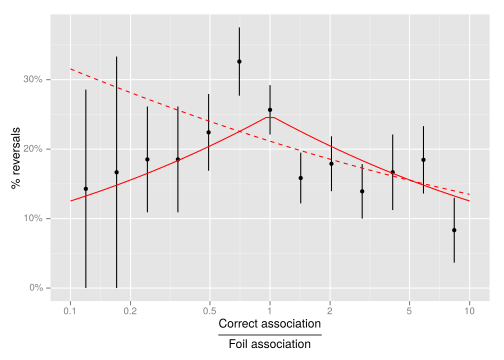
\includegraphics[width=.7\textwidth]{imgs/exp4_reversals.pdf}
  \caption[Proportion of correct responses that involved reversals,
  Experiment 4.]{
    The proportion of correct responses
    where participants initially moved towards the foil species.
    A model using the log-transformed association ratio as a predictor
    (dashed red line) showed that participants were more likely
    to produce these reversal trajectories when the association ratio
    favoured the foil species.
    However, the data were slightly better fit by a model (solid red line)
    which showed that these reversals were most likely to occur
    when the association ratio favoured neither response.
    \label{fig:exp4_reversals}
  }
\end{figure}

\begin{figure}[bp]
  \centering
  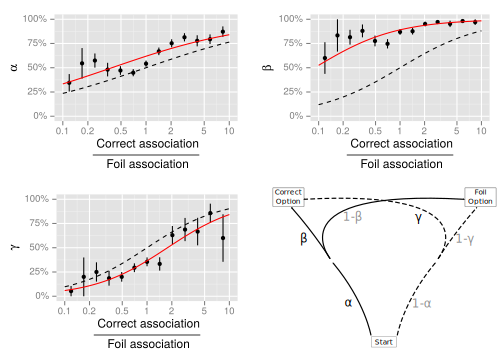
\includegraphics[width=.7\textwidth]{imgs/exp4_transitions_combined.pdf}
  \caption[Transition probabilities, as a function of the association ratio,
    in Experiment 4.]{
    \label{fig:exp4_transitions}
    Transitions probabilities from Experiment 4,
    as functions of the association ratios.
    As the association ratio increased in favour of the correct species,
    participants became more likely to initially move towards that species ($\alpha$, top left),
    to select that species after initially moving towards it ($\beta$, top right),
    and to select it even after initially moving towards the foil ($\gamma$, bottom left).
    Dashed lines show the expected values if participants were
    influenced by association ratio only.
    Overview of the three parameters can be seen in the bottom right.
  }
\end{figure}


The model for $\alpha$ (Figure~\ref{fig:exp4_transitions}, top left)
had a marginally significant positive intercept
($logit(\beta)$ = 62\%, CI = [50\%, 73\%], z = 1.886, p = .0593)
indicating that participants initially moved towards the correct species
on 62\% of trials when the ratio was $\frac{1}{1}$,
more than the 50\% that would be expected 
based on the association ratio alone.
The association ratio was also a significant positive predictor
($e^{\beta}$ = 1.7, CI = [1.4, 2.0], z = 6.109, p < .0001)
such that participants became more likely to initially move
towards the correct species as it was increasingly favoured by the association ratio.

The model for $\beta$  (Figure~\ref{fig:exp4_transitions}, top right)
had a robust positive intercept
($logit(\beta)$ = 80\%, CI = [85\%, 92\%], z = 10.567, p < .0001),
meaning that after initially moving towards the correct species,
participants selected that species 80\% of the time
when the association ratio was $\frac{1}{1}$.
The association ratio was also a significant positive predictor here
($e^{\beta}$ = 2.4, CI = [1.8, 3.2], z = 5.678, p < .0001),
meaning that participants became more likely to select the correct species
on trials where they initially moved towards it
as the association ratio in favour of the correct species increased.
In general, however, participants very rarely
changed direction after moving towards the correct species
in any case.

Finally, the model for $\gamma$  (Figure~\ref{fig:exp4_transitions}, bottom left)
contained a significant \emph{negative} intercept
($logit(\beta)$ = 37\%, CI = [30\%, 43\%], z = 3.963, p < .0001),
indicating that on trials where they initially moved towards the foil species,
participants only changed direction to select the correct species instead
37\% of the time when the association ratio was $\frac{1}{1}$.
The association ratio was again a positive predictor here
($e^{\beta}$ = 2.6, CI = [2.0, 3.5], z = 6.374, p < .0001),
meaning that as the strength of the association ratio
in favour of the correct species increased,
participants were more likely to switch direction
and select the correct species when they initially moved towards the foil.


\subsubsection{Time course}
\FloatBarrier

\begin{figure}[ht]
  \centering
  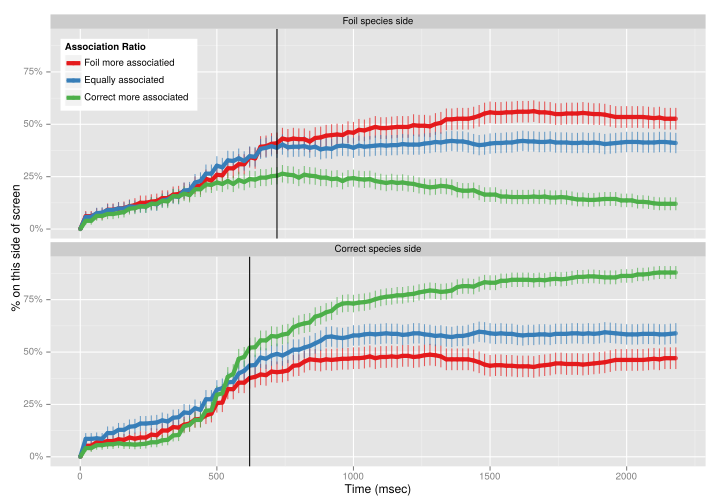
\includegraphics[width=\figurewidth]{imgs/exp4_condition_timecourse.pdf}
  \caption[Time course, separately for each response option, in Experiment 4.]{
    Proportion of trials on side of screen corresponding to the correct species (top)
    and the foil species (bottom) over time.
    The association ratio is a significant predictor
    of movements towards the foil from 720 msec,
    and of movements towards the correct species from 620 msec (solid vertical lines).
    \label{fig:exp4_condition_timecourse} }
\end{figure}


As usual, the time course of  the mouse movements here
reveals more about the points at which participants were
drawn towards each response.
Figure~\ref{fig:exp4_condition_timecourse} shows the proportion of trials
on the side of the screen corresponding to each species over time,
for trials where the association ratio favours the foil species (N = 359),
the two species were rated as equally associated (N = 397),
or the correct species was more strongly associated (N = 432).
To estimate divergence times,
I fitted two series of logistic mixed models,
one series predicting the probability of being on the foil species' side of the screen,
and one the probability of being on the correct species' side,
separately for every 20 msec time window.
Each model included the log-transformed association ratio  as a predictor,
and included random intercepts for each participant and each base species.
The divergence points were the times in each series
after which the association ratio is found to be a significant predictor.
The association ratio had a significant effect on
participants' probability of being on the foil species'
side of the screen from 720 msec,
and their probability of being on the correct species' side from 620 msec.

\begin{figure}[h]
  \centering
  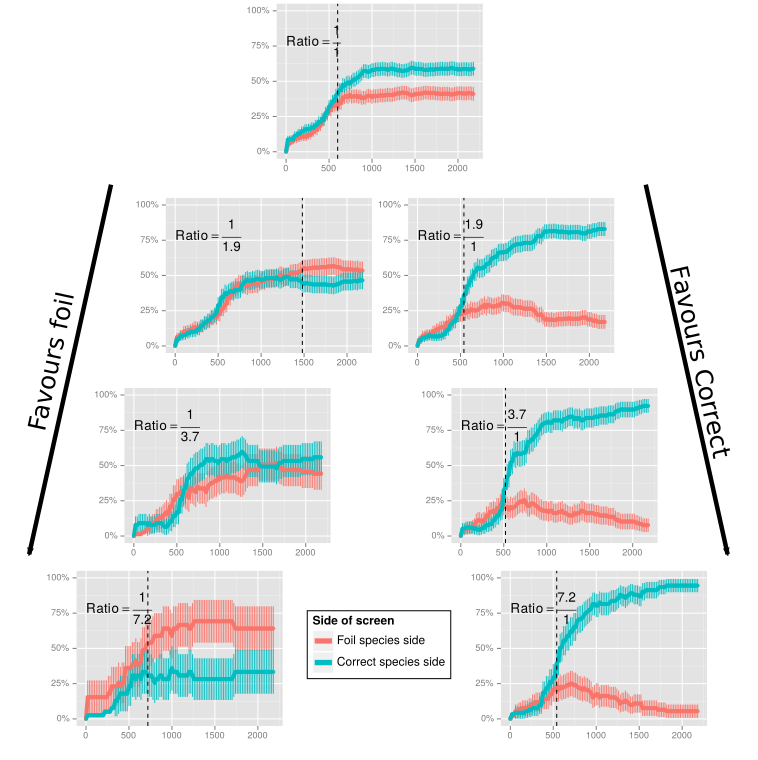
\includegraphics[width=\figurewidth]{imgs/exp4_ratio_timecourse.pdf}
  \caption[Time course, separately for different association ratios, in Experiment 4.]{
    Proportion of trials on the side of the screen corresponding to each response,
    grouped by association ratios.
    When the association ratio favours the correct option,
    %% \aside{This figure should have the divergence points marked for each trial,
    %%   a legend somewhere, and the font sizes all the same.
    %%   I will do this in the next few days when I've the use of a computer with a mouse.}
    \label{fig:exp4_ratio_timecourse} }
\end{figure}

\begin{table}
  \centering
  \caption[Divergence times, Experiment 4.]{
    Divergence times, and number of trials included,
    for each binned value of the association ratio.
    For ratios of $\frac{1}{7.2}$ and $\frac{1}{1.9}$,
    participants were significantly more likely to be on
    the foil species' side of the screen than the correct species'
    from the divergence time onwards.
    For all other ratios, participants were more likely to be on
    the correct species' side of the screen
    from the divergence time.
    \label{tab:exp4_ratio_timecourse_table}
  }
  \doublespacing
  \begin{tabular}{lrr}
    \toprule
    Ratio           & Divergence (msec) & N\\
    \midrule
    $\frac{1}{7.2}$ & 720               & 39\\
    $\frac{1}{3.7}$ & N/A               & 77\\
    $\frac{1}{1.9}$ & 1,480              & 243\\
    $\frac{1}{1}$   & 600               & 397\\
    $\frac{1.9}{1}$ & 540               & 223\\
    $\frac{3.7}{1}$ & 520               & 117\\
    $\frac{7.2}{1}$ & 540               & 92\\
    \bottomrule
  \end{tabular}
\end{table}

Figure~\ref{fig:exp4_ratio_timecourse}
shows the proportion of trials on either side of the screen,
with separate plots representing different levels of the association ratio.
For this analysis, I divided the log-transformed association ratio
into seven bins of equal width,
and labelled each bin according to the mean association ratio within it:
$\frac{1}{7.2}$, $\frac{1}{3.7}$, $\frac{1}{1.9}$, $\frac{1}{1}$, $  \frac{1.9}{1}$, $\frac{3.7}{1}$, and $\frac{7.2}{1}$.
Within each of these bins, I found the divergence point,
after which participants were more likely to be
on one side of the screen than the other,
by fitting a series of logistic mixed models,
comparing the probability of being on either side of the screen,
with random intercepts for each participant and each base species.

As the association ratio in favour of the correct species increased,
from $\frac{1}{1}$ (both species equally associated) up to $\frac{7.2}{1}$
(correct species 7.2 times more strongly associated than the foil),
we see a clear increase in the number of trials where
the cursor ends up on the correct species' side,
mirroring the earlier analysis of participants' responses.
There was little difference, however,
in the trends leading up to these final proportions.
For all of these bins, the preference for the correct species
emerged from 520 -- 600 msec,
and the shape of the curves were broadly similar,
except for the differences in their overall heights.
Thus, structured knowledge began to influence
participants' motor output from \tildetext600 msec.

When the association ratio was less than $\frac{1}{1}$, however,
and so conflicted with structured knowledge,
the trends were less clear.
When the ratio was strongest in favour of the foil species ($\frac{1}{7.2}$),
participants were more likely to move towards the foil
than the correct species from 720 msec.
Both species were equally attractive with a ratio $\frac{1}{3.7}$, however,
and with a ratio of $\frac{1}{1.9}$ a significant preference for the foil
only emerged from 1,480 msec.
Note, however, that even when the association ratio
conflicts with structured knowledge,
there is no evidence of a cross-over relationship ---
in each subplot within Figure~\ref{fig:exp4_ratio_timecourse},
participants were either drawn to the correct species, or to the foil,
but in no case were they primarily initially drawn towards the foil,
and later drawn towards the correct species.


